\setlength{\columnsep}{3pt}
\begin{flushleft}
	Commands to display all logs:
	\begin{itemize}
		\item \textbf{journalctl}: Shows the full system journal logs.
		\bigskip
		\begin{tcolorbox}[breakable,notitle,boxrule=-0pt,colback=pink,colframe=pink]
			\color{black}
			\fontdimen2\font=1em
			Syntax: journalctl [options]
			\fontdimen2\font=4pt
		\end{tcolorbox}
		Eg: 
		\begin{figure}[h!]
			\centering
			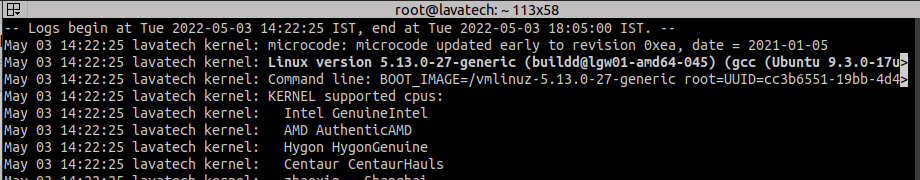
\includegraphics[scale=.35]{content/chapter16/images/journalctl.png}
			\caption{Sample output}
			\label{fig:process2346}
		\end{figure}
		
		Options with \textbf{journalctl} command:	
				
		\begin{itemize}
			\item \textbf{-p}: Display logs according to specific priority.
			\bigskip
			\begin{tcolorbox}[breakable,notitle,boxrule=-0pt,colback=pink,colframe=pink]
				\color{black}
				\fontdimen2\font=1em
				Syntax: journalctl -p priority
				\fontdimen2\font=4pt
			\end{tcolorbox}	
			Eg: 
			\begin{tcolorbox}[breakable,notitle,boxrule=-0pt,colback=black,colframe=black]
				\color{green}
				\fontdimen2\font=1em
				\#  journalctl -p err
				\fontdimen2\font=4pt
			\end{tcolorbox}

			\item \textbf{-b}: Show the log messages since the last boot of the system.
			\bigskip
			\begin{tcolorbox}[breakable,notitle,boxrule=-0pt,colback=pink,colframe=pink]
				\color{black}
				\fontdimen2\font=1em
				Syntax: journalctl -b
				\fontdimen2\font=4pt
			\end{tcolorbox}			
		
		\end{itemize}

\end{flushleft}

\newpage


